\documentclass[11pt,a4paper]{article}

\usepackage[T1]{fontenc}
\usepackage[utf8]{inputenc}
\usepackage{lmodern}
\usepackage{microtype}
\usepackage[a4paper,margin=30mm]{geometry}
\usepackage{amsmath,amssymb,amsthm,mathtools}
\usepackage{bm}
\usepackage{booktabs}
\usepackage{array}
\usepackage{enumitem}
\usepackage{xcolor}
\usepackage{listings}
\usepackage[most]{tcolorbox}
\usepackage{tikz}
\usetikzlibrary{arrows.meta,positioning}
\usepackage{xurl}
\usepackage{seqsplit}
\usepackage{needspace}
\usepackage{hyperref}
\usepackage[nameinlink,noabbrev]{cleveref}
\usepackage[numbers,sort&compress]{natbib}

\hypersetup{
  colorlinks=true,
  linkcolor=black,
  citecolor=black,
  urlcolor=black,
  pdftitle={Rooted-tree summation and Catalan closure for polymer cluster expansions with holes},
  pdfauthor={Lluis Eriksson}
}

\setlist[itemize]{leftmargin=1.5em,itemsep=0.25em,topsep=0.35em}
\setlist[enumerate]{leftmargin=1.7em,itemsep=0.25em,topsep=0.35em}
\setlength{\parindent}{1.25em}
\setlength{\parskip}{0.15em}
\allowdisplaybreaks

\newtheorem{theorem}{Theorem}[section]
\newtheorem{lemma}[theorem]{Lemma}
\newtheorem{proposition}[theorem]{Proposition}
\newtheorem{corollary}[theorem]{Corollary}
\theoremstyle{definition}
\newtheorem{definition}[theorem]{Definition}
\newtheorem{assumption}[theorem]{Assumption}
\newtheorem{remark}[theorem]{Remark}

\crefname{assumption}{Assumption}{Assumptions}
\Crefname{assumption}{Assumption}{Assumptions}

\newcommand{\supp}{\operatorname{supp}}
\newcommand{\skel}{\operatorname{skel}}
\newcommand{\Cat}{\operatorname{Cat}}
\newcommand{\Tree}{\mathcal T}
\newcommand{\Poly}{\mathcal P}
\newcommand{\Plane}{\mathcal O}
\newcommand{\eps}{\varepsilon}
\newcommand{\ind}{\mathbf 1}
\newcommand{\Hsharp}{H^{\#}}
\newcommand{\Ksharp}{K^{\#}}
\newcommand{\RR}{\mathbb R}
\newcommand{\NN}{\mathbb N}
\newcommand{\BaseCommit}{\texttt{\seqsplit{1d044a353ac2b69ddca732dd851fb0ab4a94d7af}}}
\newcommand{\LeanToolchain}{\texttt{leanprover/lean4:v4.29.0-rc6}}
\newcommand{\MathlibCommit}{\texttt{\seqsplit{07642720480157414db592fa85b626dafb71355b}}}

\DeclarePairedDelimiter{\abs}{\lvert}{\rvert}
\DeclarePairedDelimiter{\norm}{\lVert}{\rVert}
\DeclarePairedDelimiter{\set}{\lbrace}{\rbrace}

\lstdefinelanguage{Lean}{
  morekeywords={theorem,lemma,def,noncomputable,section,namespace,end,variable,open,
    import,where,by,have,show,exact,simpa,using,calc,let,fun,if,then,else,
    structure,extends,Prop,Type,forall,match,with,inductive,abbrev,example},
  sensitive=true,
  morecomment=[l]{--},
  morecomment=[s]{/-}{-/},
  morestring=[b]"
}
\lstset{
  language=Lean,
  basicstyle=\ttfamily\small,
  keywordstyle=\bfseries,
  commentstyle=\itshape,
  columns=fullflexible,
  keepspaces=true,
  breaklines=true,
  frame=single,
  framerule=0.25pt,
  xleftmargin=0.5em,
  xrightmargin=0.5em,
  aboveskip=0.7em,
  belowskip=0.7em,
  showstringspaces=false
}

\newtcolorbox{pipelinebox}{
  colback=black!2,
  colframe=black!45,
  boxrule=0.5pt,
  arc=1mm,
  left=2mm,right=2mm,top=1.5mm,bottom=1.5mm
}

\title{\bfseries Rooted-tree summation and Catalan closure for polymer cluster expansions with holes:\\a Lean 4 formalization blueprint}
\author{Llu\'is Eriksson}
\date{June 2026}

\begin{document}
\maketitle

\begin{abstract}
We isolate the combinatorial engine that converts a first polymer activity
$\Ksharp$ into the second Ursell activity $\Hsharp$ in a polymer expansion with holes.
The fixed-union condition, a marked active root, hard-core incompatibility, and the
hole-modified metric are retained until the target decay has been extracted.  The local
leaf summation for a rooted labelled tree $T$ produces the exact factor
$M^{2n+1}\prod_v c_T(v)!$, where $c_T(v)$ is the number of children of $v$ in the
root-$0$ orientation.  We prove the exact identity
\[
  \frac{1}{n!}\sum_{T\in\Tree_{n+1}}\prod_{v=0}^{n}c_T(v)! = \Cat_n
\]
by ordering the children at every vertex and identifying the resulting objects with
labelled plane rooted trees.  This replaces a geometric closure by the Catalan majorant
\[
 B_M(\eps)=\sum_{n\ge0}\Cat_nM^{2n+1}\eps^{n+1}
 =\frac{1-\sqrt{1-4M^2\eps}}{2M},
 \qquad B_M=M\eps+M B_M^2.
\]
For $0\le4M^2\eps<1$, this bound is coefficientwise sharper than
$G_M(\eps)=M\eps/(1-4M^2\eps)$.  We transport the estimate through a rooted
modified-metric profile and into the scalar one-scale remainder predicate
\texttt{SingleScaleUVDecay}.  The result specifies an Appendix-F-style
cluster-expansion mechanism and the corresponding Lean 4 theorem manifest; it does not
construct the Yang--Mills activity, a continuum limit, Osterwalder--Schrader
reconstruction, or a Yang--Mills mass gap.
\end{abstract}

\noindent\textbf{Keywords.} polymer cluster expansion; Ursell functions; rooted trees;
Catalan numbers; polymers with holes; renormalization group; Lean 4; formalization blueprint.

\medskip
\noindent\textbf{MSC 2020.} 68V20, 82B20, 05C30, 05A15.

\tableofcontents

\section{Introduction}

Cluster expansions turn a partition function into an exponential of connected
activities in abstract polymer systems \cite{KoteckyPreiss1986}.  In the presence of
holes, however, the bookkeeping has two support maps: a full target support, whose union
must remain prescribed, and an active skeleton, which controls incompatibility and
rooted summability.  Appendix~F of Dimock's presentation of the Balaban
renormalization group is a canonical source for this structure
\cite{Dimock2013LargeFields}.  Its conclusion has the schematic form
\[
  \abs{\Hsharp(Y)}
  \le C H_0\exp\!\bigl[-(\kappa-3\kappa_0-3)d_M(Y\bmod\Omega^c)\bigr],
\]
provided a small first activity is available and the hole-modified geometry is
summable.  The purpose of the present paper is not to reprove the model-specific
production of that first activity.  It is to isolate, sharpen, and state a
machine-checkable interface for the second-gas combinatorics that starts once $\Ksharp$
has been supplied.

The referenced Lean development already contains a two-support target compiler, an
integrated first activity, the second Ursell object, Penrose tree domination, a
fixed-tree leaf recursion, a geometric $4^n$ closure, rooted hole-metric summability, and
a consumer-facing one-scale remainder bridge \cite{ErikssonProgramme2026}.  Its
fixed-tree estimate is sharper than its final tree summation: for a labelled tree with
$n+1$ vertices it retains $\prod_v c_T(v)!$, but the normalized sum over tree shapes is
subsequently bounded by $4^n$.  The main observation of this manuscript is that this
last step is exactly Catalan.

\begin{pipelinebox}
\centering
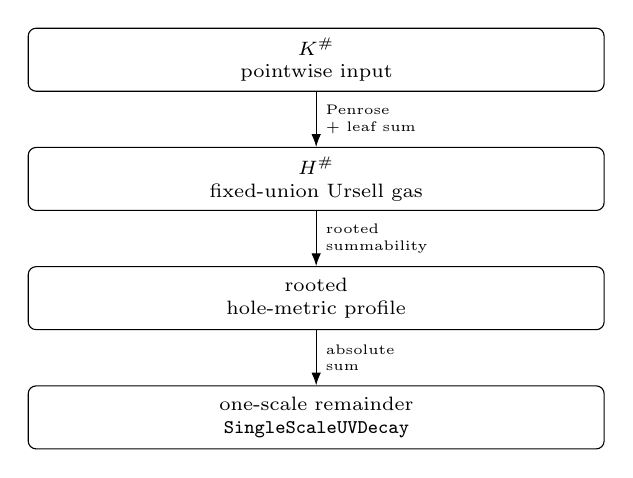
\begin{tikzpicture}[>=Latex,
  stage/.style={draw,rounded corners=1mm,minimum height=8mm,text width=0.58\linewidth,
                inner xsep=4pt,inner ysep=3pt,align=center,font=\scriptsize},
  flow/.style={->,line width=0.35pt}]
  \node[stage] (k) {$\Ksharp$\\pointwise input};
  \node[stage,below=7mm of k] (h) {$\Hsharp$\\fixed-union Ursell gas};
  \node[stage,below=7mm of h] (p) {rooted\\hole-metric profile};
  \node[stage,below=7mm of p] (r) {one-scale remainder\\\texttt{SingleScaleUVDecay}};
  \draw[flow] (k) -- node[draw=none,right,font=\tiny,align=left] {Penrose\\+ leaf sum} (h);
  \draw[flow] (h) -- node[draw=none,right,font=\tiny,align=left] {rooted\\summability} (p);
  \draw[flow] (p) -- node[draw=none,right,font=\tiny,align=left] {absolute\\sum} (r);
\end{tikzpicture}
\end{pipelinebox}

The contribution is a closure theorem rather than a new discovery about Catalan
numbers.  The identity is classical; what matters is its exact placement inside a
fixed-union expansion with holes and its transport through a reusable formal API.  The
paper proves four linked statements.

\begin{enumerate}
\item Local hard-core moment estimates imply, for every fixed rooted labelled tree, the
      factor $M^{2n+1}\prod_v c_T(v)!$ while preserving the marked root and the
      parent-edge incompatibility indicators.
\item Ordering each child fiber converts the weighted tree sum exactly into the number
      of plane rooted trees with labelled nonroot vertices.  The normalized sum is
      $\Cat_n$, not merely bounded by $4^n$.
\item The complete second-Ursell series is bounded by the square-root majorant $B_M$,
      the least nonnegative solution of $B=M\eps+MB^2$.
\item The pointwise target estimate implies a rooted profile and, under the existing
      summability hypothesis, the scalar one-scale remainder estimate used by the
      one-scale consumer predicate.
\end{enumerate}

The formalization boundary is organized so that the pure tree theorem can be reused outside the
Balaban setting.  The tree enumeration does not import gauge geometry, while the real
square-root closure does not import polymers.  This separation is important for both
mathematical clarity and artifact review.

\section{Polymers with holes and the second gas}
\label{sec:model}

We state the finite-volume theorem in an abstract form that matches the Lean interfaces.
All sums in the combinatorial part are finite.  Infinite-volume or scale-uniform
statements enter only through explicitly stated summability hypotheses.

\subsection{Two supports and a modified metric}

Let $\Lambda$ be a finite block set, let $\Omega\subseteq\Lambda$ be the active region,
and write $\Omega^c$ for the holes.  A polymer $Q\in\Poly$ carries
\begin{itemize}
\item a full support $\supp(Q)\subseteq\Lambda$;
\item a nonempty active skeleton $\skel(Q)\subseteq\Omega$;
\item a shifted hole-modified size
      $\ell(Q)=d_M(Q\bmod\Omega^c)+1\in\{1,2,\ldots\}$.
\end{itemize}
The hard-core incompatibility relation is
\[
  Q\not\sim Q' \quad\Longleftrightarrow\quad
  \skel(Q)\cap\skel(Q')\ne\varnothing.
\]
For a tuple $\bm Q=(Q_0,\ldots,Q_n)$, its prescribed full target is
\[
  U(\bm Q)=\bigcup_{i=0}^{n}\supp(Q_i).
\]
The skeleton of a representable target $Y$ is assumed to satisfy
\[
  \skel(Y)=\bigcup_{i=0}^{n}\skel(Q_i)
  \qquad\text{whenever }U(\bm Q)=Y.
\]
Thus admissibility and incompatibility use active skeletons, whereas the fiber of the
second gas uses the full union $Y$.

\begin{assumption}[Metric stitching]
\label{ass:stitch}
If the incompatibility graph of $\bm Q$ is connected and $U(\bm Q)=Y$, then
\begin{equation*}
  \ell(Y)\le \sum_{i=0}^{n}\ell(Q_i).
  \tag{S}\label{eq:stitch}
\end{equation*}
\end{assumption}

In unshifted notation, \eqref{eq:stitch} has the familiar shape
$d_M(Y)\le\sum_i d_M(Q_i)+n$.  The shift by one is useful because it makes the
multiplicative decay extraction compatible with the number of tree edges.

\subsection{First activity and local moment budgets}

Fix a residual rate $\rho\ge0$, a leaf rate $\kappa_0>0$, a small parameter
$\eps\ge0$, and a nonnegative weight $u:\Poly\to[0,\infty)$.  Assume the first
activity obeys
\begin{equation}
  \abs{\Ksharp(Q)}\le \eps\,e^{-\rho\ell(Q)}u(Q).
  \label{eq:ksharp-input}
\end{equation}
In the concrete hole geometry, $u(Q)$ is dominated by a spare exponential such as
$e^{-2\kappa_0\ell(Q)}$.  We isolate only the two consequences consumed by the tree
recursion.

\begin{assumption}[Child and root moment budgets]
\label{ass:moments}
There is $M>0$ such that, for every $j\in\NN$, every parent polymer $Q$, and every
active block $r\in\Omega$,
\begin{align*}
  \sum_{Q'\not\sim Q}
    \frac{\ell(Q')^j u(Q')}{\ell(Q)}
  &\le j!\,M^{j+1},
  \tag{C$_j$}\label{eq:child-budget}\\
  \sum_{Q:\,r\in\skel(Q)}\ell(Q)^j u(Q)
  &\le j!\,M^{j+1}.
  \tag{R$_j$}\label{eq:root-budget}
\end{align*}
\end{assumption}

The factorial dependence is the decisive feature: the moment index will become the
number of children of a tree vertex.  The repository's concrete constant is named
\path{appendixFSecondUrsellMomentConstant}.

\subsection{Ursell coefficient and exact-union activity}

Let
\[
 f(Q,Q')=-\ind[Q\not\sim Q'].
\]
For $m\ge1$, the Ursell coefficient is
\begin{equation}
 \varphi^T(Q_1,\ldots,Q_m)
 =\sum_{G\in\mathcal C_m}\prod_{\{i,j\}\in E(G)} f(Q_i,Q_j),
 \label{eq:ursell}
\end{equation}
where $\mathcal C_m$ is the set of connected simple graphs on $\{1,\ldots,m\}$.
The second-gas activity with prescribed full union is
\begin{equation}
 \Hsharp(Y)
 =\sum_{m\ge1}\frac{1}{m!}
   \sum_{\substack{(Q_1,\ldots,Q_m)\in\Poly^m\\
                   \bigcup_i\supp(Q_i)=Y}}
   \varphi^T(Q_1,\ldots,Q_m)\prod_{i=1}^{m}\Ksharp(Q_i).
 \label{eq:hsharp}
\end{equation}
Write $m=n+1$ and denote the corresponding order by $\Hsharp_n(Y)$.

The hard-core tree-graph inequality gives
\begin{equation}
 \abs{\varphi^T(Q_0,\ldots,Q_n)}
 \le \sum_{T\in\Tree_{n+1}}
     \prod_{\{i,j\}\in E(T)}\ind[Q_i\not\sim Q_j],
 \label{eq:penrose}
\end{equation}
where $\Tree_{n+1}$ is the set of labelled spanning trees on
$\{0,1,\ldots,n\}$.  We use only this inequality; sharper Penrose partition schemes
remain compatible with the argument \cite{Brydges1986,FernandezProcacci2007}.

\section{Preserving the target and marking a root}
\label{sec:root}

The order of the estimates is essential.  We first retain the exact-union condition,
use it to extract target decay, and only then enlarge the fiber to a root-marked sum over
all tuples.

\begin{lemma}[Target decay before overcounting]
\label{lem:target-decay}
Let $T\in\Tree_{n+1}$ and suppose all its parent-edge incompatibility indicators are
nonzero.  If $U(\bm Q)=Y$, then
\[
  \prod_{i=0}^{n}e^{-\rho\ell(Q_i)}u(Q_i)
  \le e^{-\rho\ell(Y)}\prod_{i=0}^{n}u(Q_i).
\]
\end{lemma}

\begin{proof}
The nonzero tree indicators make the incompatibility graph connected.
Assumption~\ref{ass:stitch} gives $\ell(Y)\le\sum_i\ell(Q_i)$.  Since $\rho\ge0$,
$e^{-\rho\sum_i\ell(Q_i)}\le e^{-\rho\ell(Y)}$.
\end{proof}

Choose $r\in\skel(Y)$.  Every tuple in the exact-union fiber satisfies
\begin{equation}
  1\le\sum_{i=0}^{n}\ind[r\in\skel(Q_i)].
  \label{eq:root-marker}
\end{equation}
The summand in \eqref{eq:penrose} is invariant under simultaneous relabelling of the
tuple and tree.  All $n+1$ marked coordinates therefore contribute equally, and
\[
  \frac{n+1}{(n+1)!}=\frac1{n!}.
\]
After this step the marked coordinate may be placed at label $0$, and the exact-union
restriction may be dropped because all remaining terms are nonnegative.  The target
factor $e^{-\rho\ell(Y)}$ has already been extracted.

\begin{proposition}[Rooted reduction of a fixed order]
\label{prop:rooted-reduction}
For $r\in\skel(Y)$,
\begin{equation}
 e^{\rho\ell(Y)}\abs{\Hsharp_n(Y)}
 \le \frac{\eps^{n+1}}{n!}
    \sum_{T\in\Tree_{n+1}} S_T(r),
 \label{eq:rooted-reduction}
\end{equation}
where, orienting $T$ away from root $0$ and writing $p_T(v)$ for the parent of
$v\ne0$,
\begin{equation}
 S_T(r)=
 \sum_{\substack{(Q_0,\ldots,Q_n)\in\Poly^{n+1}\\r\in\skel(Q_0)}}
 \left(\prod_{v\ne0}\ind[Q_{p_T(v)}\not\sim Q_v]\right)
 \prod_{v=0}^{n}u(Q_v).
 \label{eq:fixed-tree-sum}
\end{equation}
\end{proposition}

\begin{proof}
Insert \eqref{eq:ksharp-input} and \eqref{eq:penrose} into the definition of
$\Hsharp_n(Y)$.  Apply \cref{lem:target-decay}, insert the marker
\eqref{eq:root-marker}, use simultaneous permutation invariance to move the marked
coordinate to $0$, and finally forget the exact-union condition.  The normalization is
$1/n!$.
\end{proof}

At this point target, root, incompatibility, and holes have been handled without
conflation: the target survives through its extracted decay, the root remains pinned,
and every tree edge still carries the genuine active-skeleton incompatibility indicator.

\section{Fixed-tree leaf summation}
\label{sec:leaf}

For $T\in\Tree_{n+1}$ let $c_T(v)$ be the number of children of $v$ in the root-$0$
orientation.  Then
\begin{equation}
  \sum_{v=0}^{n}c_T(v)=n.
  \label{eq:child-sum}
\end{equation}

\begin{theorem}[Fixed-tree factorial-moment bound]
\label{thm:fixed-tree}
Under Assumption~\ref{ass:moments}, for every $T\in\Tree_{n+1}$ and every active root
$r$,
\begin{equation}
  S_T(r)\le M^{2n+1}\prod_{v=0}^{n}c_T(v)!.
  \label{eq:fixed-tree-bound}
\end{equation}
\end{theorem}

\begin{proof}
Write $\ell_v=\ell(Q_v)$.  Parent fibers satisfy the exact cancellation identity
\begin{equation}
 \prod_{v\ne0}\ell_{p_T(v)}
 =\prod_{v=0}^{n}\ell_v^{c_T(v)}.
 \label{eq:metric-cancellation}
\end{equation}
Therefore the summand in \eqref{eq:fixed-tree-sum} can be rewritten as
\begin{equation}
 \left[
  \prod_{v\ne0}
   \frac{\ell_v^{c_T(v)}u(Q_v)
         \ind[Q_{p_T(v)}\not\sim Q_v]}
        {\ell_{p_T(v)}}
 \right]
 \ell_0^{c_T(0)}u(Q_0).
 \label{eq:normalized-product}
\end{equation}
Sum the nonroot variables from the leaves toward the root.  At a nonroot vertex $v$,
with its parent polymer fixed, the corresponding normalized kernel is bounded by
\eqref{eq:child-budget} with $j=c_T(v)$:
\[
  \sum_{Q_v\not\sim Q_{p_T(v)}}
    \frac{\ell(Q_v)^{c_T(v)}u(Q_v)}{\ell(Q_{p_T(v)})}
  \le c_T(v)!M^{c_T(v)+1}.
\]
After all nonroot variables are eliminated, the root sum is bounded by
\eqref{eq:root-budget} with $j=c_T(0)$:
\[
  \sum_{Q_0:\,r\in\skel(Q_0)}
     \ell(Q_0)^{c_T(0)}u(Q_0)
  \le c_T(0)!M^{c_T(0)+1}.
\]
Multiplying the vertex budgets yields
\[
  S_T(r)
  \le \left(\prod_v c_T(v)!\right)
       M^{\sum_v(c_T(v)+1)}.
\]
By \eqref{eq:child-sum}, the exponent is $n+(n+1)=2n+1$.
\end{proof}

\begin{remark}[Why the factorial is structural]
The factor $c_T(v)!$ is not a coarse tree-count artifact.  It is the exact price of the
$c_T(v)$-th metric moment generated when the descendants of $v$ have been summed.  The
remaining combinatorial problem is precisely to evaluate these factorial products over
labelled tree shapes.
\end{remark}

Combining \cref{prop:rooted-reduction,thm:fixed-tree} gives
\begin{equation}
 e^{\rho\ell(Y)}\abs{\Hsharp_n(Y)}
 \le \eps^{n+1}M^{2n+1}
    \left(\frac1{n!}\sum_{T\in\Tree_{n+1}}\prod_v c_T(v)!\right).
 \label{eq:before-catalan}
\end{equation}
Everything specific to holes is now confined to $M$, the target length $\ell(Y)$, and
the existence of $r\in\skel(Y)$.  The parenthesized expression is pure enumerative
combinatorics.

\section{The exact rooted-tree identity}
\label{sec:catalan-identity}

Let $\Plane_n$ denote the set of plane rooted tree shapes with $n$ edges.  It is
classical that
\begin{equation}
  \abs{\Plane_n}=\Cat_n=\frac{1}{n+1}\binom{2n}{n};
  \label{eq:catalan-count}
\end{equation}
for example, by the first-child/next-sibling correspondence with binary trees or the
contour-word bijection with Dyck paths \cite{Stanley1999,FlajoletSedgewick2009}.

\begin{theorem}[Rooted child-factorial identity]
\label{thm:tree-catalan}
For every $n\ge0$,
\begin{equation}
  \boxed{
  \frac1{n!}\sum_{T\in\Tree_{n+1}}\prod_{v=0}^{n}c_T(v)! = \Cat_n.}
  \label{eq:tree-catalan}
\end{equation}
Equivalently,
\[
  \sum_{T\in\Tree_{n+1}}\prod_v c_T(v)! = n!\Cat_n.
\]
\end{theorem}

\begin{proof}
For a rooted labelled tree $T$, independently choose a linear order on the children of
each vertex.  Since the child set of $v$ has cardinality $c_T(v)$, the number of order
assignments is $\prod_v c_T(v)!$.  Thus the unnormalized left-hand side counts pairs
\[
 \mathfrak D_n=
 \set{(T,(\prec_v)_{v=0}^{n}):
       T\in\Tree_{n+1},\ \prec_v\text{ linearly orders the children of }v}.
\]
Orienting $T$ away from $0$ and using the chosen child orders turns such a pair into a
plane rooted tree whose vertices are labelled by $\{0,1,\ldots,n\}$ and whose root has
label $0$.  Conversely, forgetting the plane embedding recovers $T$, while the
left-to-right child orders recover every $\prec_v$.  This is a bijection.

Now forget the nonroot labels.  Every shape in $\Plane_n$ has $n$ nonroot vertex
positions, which can be labelled bijectively by $\{1,\ldots,n\}$ in exactly $n!$ ways;
the root label is fixed.  Consequently
\[
  \abs{\mathfrak D_n}=n!\abs{\Plane_n}=n!\Cat_n.
\]
\end{proof}

\begin{remark}[Formalization-friendly factorization]
A Lean proof may factor the bijection into three reusable equivalences: a tree together
with one permutation of every finite child fiber is a labelled ordered rooted tree;
first-child/next-sibling turns an ordered rooted tree with $n$ nonroot vertices into a
binary tree with $n$ nodes; fixing the root label leaves $n!$ labelings.  Mathlib already
supplies Catalan numbers, finite permutation cardinalities, and a Catalan cardinality
theorem for binary trees \cite{MathlibCatalan}.
\end{remark}

\begin{corollary}[Exact improvement over the profile count]
\label{cor:central-binomial}
The normalized tree sum obeys
\[
 \Cat_n=\frac{1}{n+1}\binom{2n}{n}
 \le\binom{2n}{n}\le4^n.
\]
Thus a parent-map profile overcount loses an explicit factor $n+1$, and the subsequent
geometric bound discards the polynomial decay of the Catalan coefficients.
\end{corollary}

\section{Catalan closure and the square-root majorant}
\label{sec:closure}

For $M>0$ and $\eps\ge0$, define
\begin{equation}
  B_M(\eps)
  :=\sum_{n=0}^{\infty}\Cat_n M^{2n+1}\eps^{n+1}
  =M\eps\sum_{n=0}^{\infty}\Cat_n(M^2\eps)^n.
  \label{eq:B-series}
\end{equation}
Let $C(x)=\sum_{n\ge0}\Cat_nx^n$.  The Catalan recurrence gives $C=1+xC^2$.  For
$0\le x<1/4$, the branch with $C(0)=1$ is
\begin{equation}
  C(x)=\frac{1-\sqrt{1-4x}}{2x}
      =\frac{2}{1+\sqrt{1-4x}},
  \label{eq:C-closed}
\end{equation}
where the second expression also covers $x=0$ directly.

\begin{theorem}[Square-root closure]
\label{thm:square-root}
Let $M>0$ and $0\le4M^2\eps<1$.  Then \eqref{eq:B-series} converges and
\begin{equation}
 \boxed{
  B_M(\eps)=\frac{1-\sqrt{1-4M^2\eps}}{2M}.}
 \label{eq:B-closed}
\end{equation}
Moreover,
\begin{equation}
  B_M(\eps)=M\eps+M B_M(\eps)^2,
  \label{eq:B-fixed-point}
\end{equation}
and $B_M(\eps)$ is the least nonnegative solution of this fixed-point equation.
\end{theorem}

\begin{proof}
Set $x=M^2\eps$ in \eqref{eq:C-closed} and multiply by $M\eps$, yielding
\eqref{eq:B-closed}.  Multiplying $C=1+xC^2$ by $M\eps$ gives
\[
 B_M=M\eps+M(M\eps C(x))^2=M\eps+MB_M^2.
\]
The quadratic $Mb^2-b+M\eps=0$ has roots
$(1\pm\sqrt{1-4M^2\eps})/(2M)$.  The minus branch is nonnegative, tends to zero with
$\eps$, and is no larger than the plus branch.
\end{proof}

\begin{corollary}[Linear small-activity bound]
\label{cor:linear-B}
If $M>0$ and $0\le4M^2\eps\le1$, then
\begin{equation}
  0\le B_M(\eps)
  =\frac{2M\eps}{1+\sqrt{1-4M^2\eps}}
  \le2M\eps.
  \label{eq:B-linear}
\end{equation}
\end{corollary}

The numerical Catalan series also converges at $4M^2\eps=1$ and has value $1/(2M)$.
We use a strict interior condition below because independent source interfaces often
impose strict smallness.  Boundary convergence of the Catalan series should not be
confused with boundary validity of every model-specific analytic input.

\subsection{Explicit comparison with the geometric majorant}

The geometric closure obtained from the bound $\Cat_n\le4^n$ is
\begin{equation}
  G_M(\eps)
  :=\sum_{n=0}^{\infty}4^nM^{2n+1}\eps^{n+1}
  =\frac{M\eps}{1-4M^2\eps},
  \qquad 0\le4M^2\eps<1.
  \label{eq:G}
\end{equation}

\begin{proposition}[Catalan versus geometric closure]
\label{prop:B-vs-G}
For $M>0$ and $0\le4M^2\eps<1$,
\begin{equation}
  B_M(\eps)\le G_M(\eps),
  \label{eq:B-le-G}
\end{equation}
with strict inequality for $\eps>0$.  Coefficientwise,
\[
 \begin{array}{rcl}
 B_M(\eps)&=&M\eps+M^3\eps^2+2M^5\eps^3+5M^7\eps^4+\cdots,\\[1mm]
 G_M(\eps)&=&M\eps+4M^3\eps^2+16M^5\eps^3+64M^7\eps^4+\cdots.
 \end{array}
\]
As $4M^2\eps\uparrow1$, $B_M(\eps)\to1/(2M)$ while $G_M(\eps)\to+\infty$.
\end{proposition}

\begin{proof}
The coefficientwise inequality is $\Cat_n\le4^n$.  It is strict for every $\eps>0$
because $\Cat_1=1<4$.  The limiting statements follow from \eqref{eq:B-closed} and
\eqref{eq:G}.
\end{proof}

The Catalan replacement changes neither the fixed-tree moment constant $M$, nor the
target rate, nor the hole geometry.  It changes only the final universal shape sum.

\section{From \texorpdfstring{$\Ksharp$}{K-sharp} to \texorpdfstring{$\Hsharp$}{H-sharp}}
\label{sec:k-to-h}

\begin{theorem}[Catalan second-gas bound with prescribed union]
\label{thm:k-to-h}
Assume the metric stitching and moment hypotheses, \cref{ass:stitch,ass:moments},
together with the pointwise first-activity estimate \eqref{eq:ksharp-input}.  Let $Y$
be a representable nonempty target and choose
$r\in\skel(Y)$.  If $M>0$ and $0\le4M^2\eps<1$, then the second Ursell series
\eqref{eq:hsharp} is absolutely convergent and
\begin{equation}
  \boxed{
  \abs{\Hsharp(Y)}\le B_M(\eps)e^{-\rho\ell(Y)}.}
  \label{eq:H-pointwise}
\end{equation}
At fixed order,
\begin{equation}
  \abs{\Hsharp_n(Y)}
  \le \Cat_nM^{2n+1}\eps^{n+1}e^{-\rho\ell(Y)}.
  \label{eq:H-order}
\end{equation}
\end{theorem}

\begin{proof}
Insert \cref{thm:tree-catalan} into \eqref{eq:before-catalan} to obtain
\eqref{eq:H-order}.  Summing over $n\ge0$ gives \eqref{eq:H-pointwise} by the
definition of $B_M$ and proves absolute convergence.
\end{proof}

\begin{corollary}[Appendix-F residual-rate form]
\label{cor:appendix-f-rate}
Suppose the decay split in the first activity yields
\[
  \rho=\kappa-3\kappa_0-3,
  \qquad \kappa\ge3\kappa_0+3.
\]
Then $\rho\ge0$ and
\[
  \abs{\Hsharp(Y)}
  \le B_M(\eps)
      \exp\!\bigl[-(\kappa-3\kappa_0-3)
                    (d_M(Y\bmod\Omega^c)+1)\bigr].
\]
In particular, \cref{cor:linear-B} gives
\[
  \abs{\Hsharp(Y)}\le2M\eps e^{-\rho\ell(Y)}.
\]
\end{corollary}

The statement preserves the Appendix-F structure: the union is exactly $Y$,
incompatibility is active-skeleton overlap, and decay is measured in the metric with
holes contracted.  Only after those facts have been used does the proof pass to a
root-marked overcount.

\section{Rooted profile and one-scale remainder}
\label{sec:profile}

A pointwise activity estimate becomes useful to a renormalization-group consumer after
it has been summed in a local window.  Let $a\in\Omega$ and, for
$0\le\lambda\le\rho$, define
\begin{equation}
  \mathcal P_a^{\lambda}(F)
  :=\sum_{Y:\,a\in\skel(Y)}e^{\lambda\ell(Y)}\abs{F(Y)}.
  \label{eq:root-profile}
\end{equation}

\begin{assumption}[Rooted hole-metric summability]
\label{ass:root-sum}
For some $\kappa_0>0$ and $K_0<\infty$,
\begin{equation}
  \sup_{a\in\Omega}
  \sum_{Y:\,a\in\skel(Y)}e^{-\kappa_0\ell(Y)}\le K_0.
  \label{eq:root-sum}
\end{equation}
\end{assumption}

\begin{corollary}[Rooted Catalan profile]
\label{cor:rooted-profile}
Under the hypotheses of \cref{thm:k-to-h,ass:root-sum}, if $\rho\ge\kappa_0$, then
\begin{equation}
  \sup_{a\in\Omega}\mathcal P_a^{\rho-\kappa_0}(\Hsharp)
  \le K_0 B_M(\eps).
  \label{eq:rooted-profile-bound}
\end{equation}
\end{corollary}

\begin{proof}
By \eqref{eq:H-pointwise},
\[
 e^{(\rho-\kappa_0)\ell(Y)}\abs{\Hsharp(Y)}
 \le B_M(\eps)e^{-\kappa_0\ell(Y)}.
\]
Sum over targets rooted at $a$ and apply \eqref{eq:root-sum}.
\end{proof}

For the residual rate $\rho=\kappa-3\kappa_0-3$, the sufficient margin
$\rho\ge\kappa_0$ is $\kappa\ge4\kappa_0+3$.  This is stronger than the
nonnegativity condition $\kappa\ge3\kappa_0+3$.  The stronger margin is needed only
when a summability theorem proved at exponent $\kappa_0$ is reused; a direct theorem at
the residual exponent avoids this loss.

Let $t,k\in\NN$ be scale indices, let $g(k)\ge0$, and let $a_{t,k}$ be the root selected
by the one-scale construction.  Suppose the scalar remainder is
\begin{equation}
  R_{\mathrm{sc}}(t,k)
  =\sum_{Y:\,a_{t,k}\in\skel(Y)}
      \pi\bigl(\Hsharp_{t,k}(Y)\bigr),
  \qquad \abs{\pi(z)}\le\abs{z}.
  \label{eq:remainder-def}
\end{equation}

\begin{definition}[Consumer-facing one-scale decay]
The predicate \texttt{SingleScaleUVDecay} means that
\begin{equation}
  \abs{R_{\mathrm{sc}}(t,k)}
  \le A e^{-c_0t}g(k)^{\kappa_0}
  \qquad\text{for every }t,k\in\NN.
  \label{eq:ssuv}
\end{equation}
\end{definition}

\begin{theorem}[Catalan profile to a one-scale remainder]
\label{thm:single-scale}
For every $t,k$, assume the hypotheses of \cref{thm:k-to-h} with smallness parameter
$\eps_{t,k}$ and a common moment constant $M$.  Assume also \cref{ass:root-sum} and
\[
  B_M(\eps_{t,k})\le A e^{-c_0t}g(k)^{\kappa_0}.
  \label{eq:closed-scale-comparison}
\]
If \eqref{eq:remainder-def} is absolutely summable, then
\begin{equation}
  \abs{R_{\mathrm{sc}}(t,k)}
  \le AK_0e^{-c_0t}g(k)^{\kappa_0}.
  \label{eq:remainder-bound}
\end{equation}
Thus \texttt{SingleScaleUVDecay} holds with amplitude $AK_0$.
\end{theorem}

\begin{proof}
Use the contraction property of $\pi$, absolute convergence, and
\eqref{eq:rooted-profile-bound} with zero or nonnegative tilt:
\[
 \abs{R_{\mathrm{sc}}(t,k)}
 \le\sum_{Y:\,a_{t,k}\in\skel(Y)}\abs{\Hsharp_{t,k}(Y)}
 \le K_0B_M(\eps_{t,k}).
\]
Then apply \eqref{eq:closed-scale-comparison}.
\end{proof}

This is the requested pipeline
\[
  \Ksharp\longrightarrow\Hsharp
  \longrightarrow\text{rooted profile}
  \longrightarrow\text{one-scale remainder}.
\]
The first arrow contains the Catalan closure; the later arrows are norm and summability
transports and therefore remain unchanged when the geometric majorant is replaced.

\section{Lean 4 formalization architecture}
\label{sec:lean}

Lean 4 and mathlib provide the proof-assistant substrate
\cite{deMouraLean2015,Mathlib2020}.  The proposed formalization is a conservative extension of
the base repository state listed in \cref{sec:repro}.  The base chain already establishes
the exact finite fixed-tree estimate and then closes it using $4^n$.  The Catalan patch
is intended to replace only that universal shape theorem and add the square-root
analytic consumer.

\subsection{Existing verified substrate}

\begin{table}[ht]
\centering
\footnotesize
\begin{tabular}{>{\raggedright\arraybackslash}p{0.35\textwidth}
                >{\raggedright\arraybackslash}p{0.56\textwidth}}
\toprule
Module & Role in the proof \\
\midrule
\texttt{KP/RootedChildCount}
 & Child fibers, $\sum_v c_T(v)=n$, factorial products, and explicit child-order assignments. \\
\texttt{KP/RootedLeafSummation}
 & Current parent-profile and $4^n$ aggregate tree bounds; this is the replacement point. \\
\texttt{RG/SecondUrsellLeafSummation}
 & Hard-core moment kernels, exact metric cancellation, fixed-tree bound
   $M^{2n+1}\prod_v c_T(v)!$, and current geometric leaf closure. \\
\texttt{RG/AppendixFHsharp*}
 & Fixed-union $\Hsharp$, tree domination, source majorants, profiles, convergence, and residual adapters. \\
\texttt{RG/ClusterWithHolesBridge}
 & Rooted modified-metric summability and residual-rate aggregation. \\
\texttt{RG/SingleScaleUVDecay}
 & Absolute activity sum to the scalar one-scale consumer predicate. \\
\bottomrule
\end{tabular}
\caption{Existing formal substrate consumed by the Catalan patch.}
\label{tab:modules}
\end{table}

The fixed-tree result corresponding to \cref{thm:fixed-tree} has the following shape.
\begin{lstlisting}
theorem
  fixedParentKernelSum_le_childFactor_mul_momentPow ... :
  fixedParentKernelSum ... T <=
    (Finset.univ.prod fun v : Fin (n + 1) =>
      ((KP.rootedChildCount T v).factorial : Real)) *
    appendixFSecondUrsellMomentConstant d kappa0 ^ (2 * n + 1)
\end{lstlisting}
The current aggregate step is the theorem whose name ends in
\texttt{normalized\_le\_four\_pow}.  The exact theorem has the same left-hand side
and changes only the right-hand side.

\subsection{New reusable API}

The pure-combinatorial module is proposed as
\path{YangMills/KP/RootedCatalan.lean}.  Its headline statement is:
\begin{lstlisting}
theorem rootedChildCount_factorialTreeSum_normalized_eq_catalan
    (n : Nat) :
    ((n : Real) + 1) / ((n + 1).factorial : Real) *
      (KP.spanningTrees (top : SimpleGraph (Fin (n + 1))).sum
        (fun T => Finset.univ.prod fun v : Fin (n + 1) =>
          ((KP.rootedChildCount T v).factorial : Real)))
      = (Nat.catalan n : Real)
\end{lstlisting}
Because $(n+1)/(n+1)!=1/n!$, this is exactly \eqref{eq:tree-catalan} in the
normalization already consumed by the second gas.

The analytic module defines both majorants and proves the fixed-point equation:
\Needspace{18\baselineskip}
\begin{lstlisting}
noncomputable def catalanClosure (M epsilon : Real) : Real :=
  (1 - Real.sqrt (1 - 4 * M^2 * epsilon)) / (2 * M)

noncomputable def geometricClosure (M epsilon : Real) : Real :=
  M * epsilon / (1 - 4 * M^2 * epsilon)

theorem catalanClosure_fixedPoint
    (hM : 0 < M) (hepsilon : 0 <= epsilon)
    (hsmall : 4 * M^2 * epsilon <= 1) :
    catalanClosure M epsilon =
      M * epsilon + M * (catalanClosure M epsilon)^2 := by
  have hrad : 0 <= 1 - 4 * M^2 * epsilon := by nlinarith
  have hs := Real.sq_sqrt hrad
  unfold catalanClosure
  field_simp [ne_of_gt hM]
  nlinarith
\end{lstlisting}
The formal power-series identity is independently available in mathlib as
\path{PowerSeries.catalanSeries_sq_mul_X_add_one}; the real square-root theorem belongs
in the project layer because the polymer consumer is an inequality over $\RR$.

The source theorem keeps the established target-decay extraction and leaf sum, replacing
its geometric ratio by the exact order bound
\begin{lstlisting}
appendixFHoleHsharpWeightedTreeTerm ... Y n <=
  (Nat.catalan n : Real) * M^(2*n+1) * epsilon^(n+1) *
    appendixFHoleExpWeight HF residualRate Y
\end{lstlisting}
and its total profile by \texttt{catalanClosure M epsilon}.  No definition of full
support, skeleton, incompatibility, or modified metric changes.

\subsection{Proof decomposition in Lean}

A reviewable implementation should expose the following intermediate objects rather than
hide the bijection in one opaque cardinality calculation.
\begin{enumerate}
\item \texttt{rootedChildOrderAssignments T}: one finite permutation for each child
      fiber, whose cardinality is $\prod_v c_T(v)!$.
\item A type of labelled ordered rooted trees with root label $0$ and a forgetful map to
      complete-graph spanning trees.
\item An equivalence between ordered rooted trees and a Catalan-counted tree type, such
      as binary trees under first-child/next-sibling.
\item A separation of shape and labels, proving that every unlabelled shape has exactly
      $n!$ root-preserving labelings.
\item A cast theorem from the natural-number cardinality identity to the real normalized
      identity consumed by the existing second-Ursell code.
\end{enumerate}
This decomposition makes the exact theorem reusable and gives small finite objects for
regression testing.

\subsection{Oracle discipline}

Every new headline theorem is checked with
\Needspace{8\baselineskip}
\begin{lstlisting}
#print axioms YangMills.KP.rootedChildCount_factorialTreeSum_normalized_eq_catalan
#print axioms YangMills.RG.appendixFHoleHsharpTerm_le_catalan
#print axioms YangMills.RG.singleScaleUVDecay_of_catalanProfile
\end{lstlisting}
The expected output is the standard Lean kernel footprint
\texttt{[propext, Classical.choice, Quot.sound]}, with no \texttt{sorryAx} and no
project-specific axioms.  The finite bijection is classical; use of
\texttt{Classical.choice} is expected and does not weaken kernel soundness.

\section{Reproducibility}
\label{sec:repro}

A future archival artifact should archive both the paper source and the exact repository
commit containing the Catalan patch.  The base state inspected for this manuscript is:
\begin{center}
\begin{tabular}{@{}>{\raggedright\arraybackslash}p{0.24\textwidth}>{\raggedright\arraybackslash}p{0.66\textwidth}@{}}
\toprule
Base repository commit & \BaseCommit \\
Lean toolchain & \LeanToolchain \\
mathlib commit & \MathlibCommit \\
Core target & \texttt{YangMillsCore} \\
Catalan patch status & specified here; not yet an archived Lean commit \\
\bottomrule
\end{tabular}
\end{center}

From a fresh clone, the base verification commands are:
\begin{lstlisting}[language={}]
git checkout 1d044a353ac2b69ddca732dd851fb0ab4a94d7af
lake exe cache get
lake build YangMillsCore
lake env lean oracle_check.lean
python scripts/check_consistency.py
\end{lstlisting}
Once the Catalan patch is implemented, the focused checks are:
\begin{lstlisting}[language={}]
lake env lean YangMills/KP/RootedCatalan.lean
lake env lean YangMills/RG/AppendixFHsharpCatalanClosure.lean
lake env lean YangMills/RG/AppendixFHsharpCatalanSource.lean
lake build YangMillsCore
lake env lean oracle_check.lean
python scripts/check_consistency.py
\end{lstlisting}
Any artifact that claims the Catalan patch has been formalized must record the resulting
commit rather than a moving branch.  It should also include a machine-readable theorem
manifest listing the fixed-tree lemma, exact Catalan identity, square-root closure,
pointwise $\Hsharp$ theorem, rooted profile, and final \texttt{SingleScaleUVDecay}
producer.

\begin{remark}[Status of the code claim]
The public base state cited above contains the fixed-tree child-factorial estimate and
the geometric closure.  The exact Catalan theorem and square-root downstream adapter are
the narrowly scoped patch specified by this paper.  Publication language such as
``formalized in Lean with no \texttt{sorry}'' should be used for that patch only after
the archived commit builds and its axiom report is included in the artifact.
\end{remark}

\section{What this theorem does not prove}
\label{sec:not-prove}

This section is part of the theorem statement, not a disclaimer added after the fact.
The formal result has a precise conditional scope.

\begin{enumerate}
\item \textbf{It does not produce the first activity $\Ksharp$.}
      The estimate \eqref{eq:ksharp-input}, its integrability, support properties, and
      scale dependence are inputs.  In a gauge model they must come from the actual
      fluctuation integral and localization analysis.
\item \textbf{It does not prove \texttt{hRpoly} or a model-specific gauge remainder
      theorem.}  The scalar extraction in \eqref{eq:remainder-def} must be contractive
      and must represent the physical remainder; that identification is external.
\item \textbf{It does not prove the Balaban renormalization-group construction.}
      Stability, gauge covariance, large-field control, interpolation, random-walk
      expansions, and iteration through all scales remain separate obligations.
\item \textbf{It does not derive the local moment budgets from Yang--Mills dynamics.}
      This paper proves how \eqref{eq:child-budget}--\eqref{eq:root-budget} close the tree
      sum.  Their realization with the desired physical constants must be verified in
      the concrete model.
\item \textbf{It does not take a continuum limit.}  No removal of lattice spacing or
      volume cutoff is performed here.
\item \textbf{It does not establish Osterwalder--Schrader or Wightman reconstruction.}
      Reflection positivity, Euclidean invariance in the limit, regularity, and
      reconstruction are outside the theorem.
\item \textbf{It does not prove the Yang--Mills existence and mass-gap problem.}
      The endpoint \texttt{SingleScaleUVDecay} is one conditional scalar input to a
      larger lattice argument; it is not a continuum Clay theorem.
\item \textbf{It does not certify an unarchived code claim.}  The Catalan patch is a
      formalization claim only after the exact archived commit builds, contains no
      \texttt{sorry}, and passes the stated axiom and consistency checks.
\end{enumerate}

What the theorem \emph{does} prove is correspondingly sharp: once a first activity and
the explicit local hole-geometry budgets are supplied, the complete second-Ursell
combinatorics -- prescribed union, root marking, hard-core edges, exact Catalan tree
summation, rooted profile, and scalar one-scale aggregation -- closes with the
square-root majorant.

\section{Discussion}

The identity in \cref{thm:tree-catalan} is elementary, but its exact use has three
advantages in a formal cluster expansion.  First, it exposes the real combinatorial
object generated by the leaf proof: a plane ordering at each parent, not an arbitrary
parent-map profile.  Second, it separates constants arising from geometry from the
universal tree-shape coefficients.  Third, it provides a canonical nonlinear closure,
$B=M\eps+MB^2$, that can be reused in other polymer systems.

The improvement is especially visible near the nominal geometric threshold.  The
geometric majorant has a pole, whereas the Catalan closure remains finite.  This does
not automatically enlarge a physical convergence domain because the source activity and
other analytic interfaces may impose stricter inequalities.  It does remove an
artificial divergence introduced solely by replacing $\Cat_n$ with $4^n$.

Formalization work in constructive quantum field theory is now substantial
\cite{DouglasEtAl2026}.  The contribution here is complementary: a compact,
source-shaped combinatorial kernel is connected to an existing renormalization-group
API.  The appropriate claim is neither that Catalan numbers are new nor that
Yang--Mills is solved, but that a delicate cluster-expansion pipeline has been stated at
the correct abstraction boundary and can be certified end to end once its
model-specific inputs are supplied.

\appendix

\section{A recursive proof of the Catalan identity}
\label{app:recursive}

For completeness, define
\[
  a_n=\frac1{n!}\sum_{T\in\Tree_{n+1}}\prod_v c_T(v)!.
\]
By the child-order interpretation, $a_n$ is the number of plane rooted tree shapes with
$n$ edges.  Decompose a nontrivial plane rooted tree using the standard
first-child/next-sibling binary encoding.  The root decomposition gives
\[
  a_0=1,
  \qquad
  a_{n+1}=\sum_{i=0}^{n}a_i a_{n-i}.
\]
These are the Catalan recurrence and initial value, so $a_n=\Cat_n$.  The generating
function $A(x)=\sum_{n\ge0}a_nx^n$ satisfies $A=1+xA^2$, exactly the equation used in
\cref{thm:square-root}.  This second proof is useful in Lean when a recursive ordered
tree datatype is more convenient than an explicit global bijection.

\section{First coefficients and executable sanity checks}

For small $n$, the exact weighted sums are
\begin{center}
\begin{tabular}{c@{\qquad}c@{\qquad}c@{\qquad}c}
\toprule
$n$ & $\sum_T\prod_v c_T(v)!$ & $n!\Cat_n$ & normalized value \\
\midrule
0 & 1   & 1   & 1 \\
1 & 1   & 1   & 1 \\
2 & 4   & 4   & 2 \\
3 & 30  & 30  & 5 \\
4 & 336 & 336 & 14 \\
\bottomrule
\end{tabular}
\end{center}
For $n=2$, the rooted star contributes $2$ and the two rooted paths contribute $1$ each,
giving $4=2!\Cat_2$.  These values are suitable as finite regression tests before the
general bijection theorem is invoked.

\section{Minimal theorem manifest for an archival artifact}

A reviewable release should expose at least the following declarations, with names
adapted only if the repository namespace changes:
\begin{enumerate}
\item \path{rootedChildCount_factorialTreeSum_normalized_eq_catalan};
\item \path{appendixFHoleHsharpWeightedTreeMarkedRootSum_le_catalan};
\item \path{appendixFHoleHsharpWeightedTreeTerm_le_catalan};
\item \path{catalanClosure_eq_tsum};
\item \path{catalanClosure_fixedPoint};
\item \path{catalanClosure_le_geometricClosure};
\item \path{appendixFHoleHsharp_norm_le_catalanClosure};
\item \path{rootedAppendixFHsharpProfile_of_catalanClosure};
\item \path{singleScaleUVDecay_of_catalanProfile}.
\end{enumerate}
For each declaration, \path{oracle_check.lean} should print only the kernel footprint
\texttt{[propext, Classical.choice, Quot.sound]}.

\begin{thebibliography}{99}

\bibitem[Brydges(1986)]{Brydges1986}
D.~C. Brydges.
\newblock A short course on cluster expansions.
\newblock In K.~Osterwalder and R.~Stora, editors, \emph{Critical Phenomena,
Random Systems, Gauge Theories}, pages 129--183. North-Holland, 1986.

\bibitem[Dimock(2013)]{Dimock2013LargeFields}
J.~Dimock.
\newblock The renormalization group according to Balaban -- II. Large fields.
\newblock \emph{Journal of Mathematical Physics}, 54:092301, 2013.
\newblock doi:10.1063/1.4821275; arXiv:1212.5562.

\bibitem[Douglas et~al.(2026)Douglas, Hoback, Mei, and Nissim]{DouglasEtAl2026}
M.~R. Douglas, S.~Hoback, A.~Mei, and R.~Nissim.
\newblock Formalization of quantum field theory.
\newblock arXiv:2603.15770, 2026.

\bibitem[Eriksson(2026)]{ErikssonProgramme2026}
L.~Eriksson.
\newblock \emph{The Eriksson Programme: Lean 4 formalization repository}.
\newblock Base snapshot \texttt{1d044a353ac2b69ddca732dd851fb0ab4a94d7af}, 2026.

\bibitem[Fern\'andez and Procacci(2007)]{FernandezProcacci2007}
R.~Fern\'andez and A.~Procacci.
\newblock Cluster expansion for abstract polymer models: new bounds from an old approach.
\newblock \emph{Communications in Mathematical Physics}, 274:123--140, 2007.
\newblock doi:10.1007/s00220-007-0279-2; arXiv:math-ph/0605041.

\bibitem[Flajolet and Sedgewick(2009)]{FlajoletSedgewick2009}
P.~Flajolet and R.~Sedgewick.
\newblock \emph{Analytic Combinatorics}.
\newblock Cambridge University Press, 2009.

\bibitem[Koteck\'y and Preiss(1986)]{KoteckyPreiss1986}
R.~Koteck\'y and D.~Preiss.
\newblock Cluster expansion for abstract polymer models.
\newblock \emph{Communications in Mathematical Physics}, 103:491--498, 1986.
\newblock doi:10.1007/BF01211762.

\bibitem[de Moura et~al.(2015)de Moura, Kong, Avigad, van Doorn, and von Raumer]{deMouraLean2015}
L.~de Moura, S.~Kong, J.~Avigad, F.~van Doorn, and J.~von Raumer.
\newblock The Lean theorem prover (system description).
\newblock In \emph{CADE-25}, LNCS 9195, pages 378--388. Springer, 2015.

\bibitem[Stanley(1999)]{Stanley1999}
R.~P. Stanley.
\newblock \emph{Enumerative Combinatorics, Volume 2}.
\newblock Cambridge University Press, 1999.

\bibitem[The mathlib Community(2020)]{Mathlib2020}
The mathlib Community.
\newblock The Lean mathematical library.
\newblock In \emph{CPP 2020}, pages 367--381. ACM, 2020.

\bibitem[The mathlib Community(2026)]{MathlibCatalan}
The mathlib Community.
\newblock Catalan-number, tree-enumeration, and power-series modules.
\newblock Online mathlib4 documentation, accessed 2026.

\end{thebibliography}

\end{document}
